\documentclass[tikz,border=2pt]{standalone}
\usepackage{amsmath}
\usepackage{pgfplots}
\pgfplotsset{compat=1.18}
\usetikzlibrary{arrows.meta}
\begin{document}
% Log link: mu = exp(x^T beta). Intercept log 0.1 gives mu = 0.1; adding the binary coefficient log 1.5
% shifts the linear predictor by log 1.5 and multiplies the mean by 1.5, to 0.15.
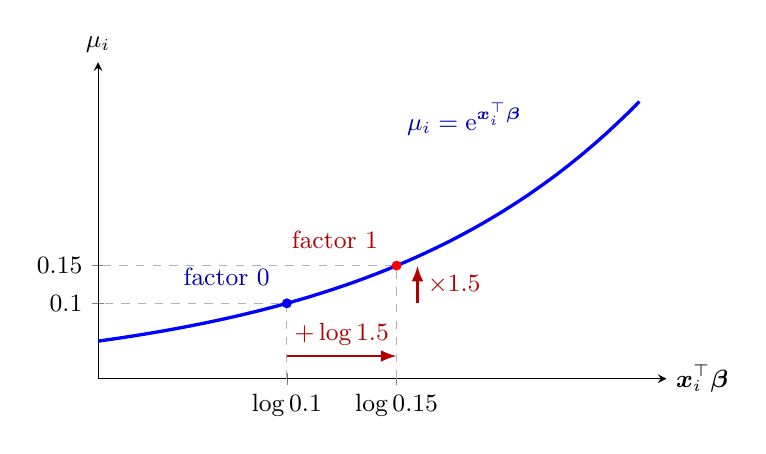
\begin{tikzpicture}[font=\small, >={Latex[length=2mm]}]
  \begin{axis}[
    axis lines=left, xmin=-3, xmax=-0.9, ymin=0, ymax=0.42,
    xtick={-2.302585,-1.89712}, xticklabels={$\log0.1$,$\log0.15$},
    ytick={0.1,0.15}, yticklabels={$0.1$,$0.15$},
    xlabel={$\boldsymbol{x}_i^{\top}\boldsymbol{\beta}$}, ylabel={$\mu_i$},
    xlabel style={at={(axis description cs:1,0)}, anchor=west},
    ylabel style={rotate=-90, at={(axis description cs:0,1)}, anchor=south},
    samples=100, width=8.8cm, height=5.6cm, clip=false]
    \addplot[blue, very thick, domain=-3:-1] {exp(x)};
    \draw[gray!60, thin, dashed] (axis cs:-2.302585,0) -- (axis cs:-2.302585,0.1) -- (axis cs:-3,0.1);
    \draw[gray!60, thin, dashed] (axis cs:-1.89712,0) -- (axis cs:-1.89712,0.15) -- (axis cs:-3,0.15);
    \fill[blue] (axis cs:-2.302585,0.1) circle (1.8pt);
    \fill[red] (axis cs:-1.89712,0.15) circle (1.8pt);
    \draw[red!70!black, ->, thick] (axis cs:-2.302585,0.03) -- node[above] {$+\log1.5$} (axis cs:-1.89712,0.03);
    \draw[red!70!black, ->, thick] (axis cs:-1.82,0.1) -- node[right] {$\times1.5$} (axis cs:-1.82,0.15);
    \node[blue!70!black, anchor=south east] at (axis cs:-2.33,0.11) {factor $0$};
    \node[red!70!black, anchor=south east] at (axis cs:-1.93,0.16) {factor $1$};
    \node[blue!70!black, anchor=south east] at (axis cs:-1.4,0.31) {$\mu_i=\mathrm{e}^{\boldsymbol{x}_i^{\top}\boldsymbol{\beta}}$};
  \end{axis}
\end{tikzpicture}
\end{document}
